
\documentclass[letterpaper,hide notes,xcolor={table,svgnames},pdftex,10pt]{beamer}
\def\showexamples{t}


%\usepackage[svgnames]{xcolor}

%% Demo talk
%\documentclass[letterpaper,notes=show]{beamer}

\usecolortheme{crane}
\setbeamertemplate{navigation symbols}{}

\usetheme{MyPittsburgh}
%\usetheme{Frankfurt}

%\usepackage{tipa}

\usepackage{hyperref}
\usepackage{graphicx,xspace}
\usepackage[normalem]{ulem}
\usepackage{multicol}
\usepackage{amsmath,amssymb,amsthm,graphicx,xspace}
\newcommand\SF[1]{$\bigstar$\footnote{SF: #1}}

\usepackage[default]{sourcesanspro}
\usepackage[T1]{fontenc}
\usepackage[scaled]{beramono}
\usepackage{tikzpagenodes}

\newcounter{tmpnumSlide}
\newcounter{tmpnumNote}


% old question code
%\newcommand\question[1]{{$\bigstar$ \small \onlySlide{2}{#1}}}
% \newcommand\nquestion[1]{\ifdefined \presentationonly \textcircled{?} \fi \note{\par{\Large \textbf{?}} #1}}
% \newcommand\nanswer[1]{\note{\par{\Large \textbf{A}} #1}}


 \newcommand\mnote[1]{%
   \addtocounter{tmpnumSlide}{1}
   \ifdefined\showcues {~\tiny\fbox{\arabic{tmpnumSlide}}}\fi
   \note{\setlength{\parskip}{1ex}\addtocounter{tmpnumNote}{1}\textbf{\Large \arabic{tmpnumNote}:} {#1\par}}}

\newcommand\mmnote[1]{\note{\setlength{\parskip}{1ex}#1\par}}

%\newcommand\mnote[2][]{\ifdefined\handoutwithnotes {~\tiny\fbox{#1}}\fi
% \note{\setlength{\parskip}{1ex}\textbf{\Large #1:} #2\par}}

%\newcommand\mnote[2][]{{\tiny\fbox{#1}} \note{\setlength{\parskip}{1ex}\textbf{\Large #1:} #2\par}}

\newcommand\mquestion[2]{{~\color{red}\fbox{?}}\note{\setlength{\parskip}{1ex}\par{\Large \textbf{?}} #1} \note{\setlength{\parskip}{1ex}\par{\Large \textbf{A}} #2\par}\ifdefined \presentationonly \pause \fi}

\newcommand\blackboard[1]{%
\ifdefined   \showblackboard
  {#1}
  \else {\begin{center} \fbox{\colorbox{blue!30}{%
         \begin{minipage}{.95\linewidth}%
           \hspace{\stretch{1}} Some space intentionally left blank; done at the blackboard.%
         \end{minipage}}}\end{center}}%
         \fi%
}



%\newcommand\q{\tikz \node[thick,color=black,shape=circle]{?};}
%\newcommand\q{\ifdefined \presentationonly \textcircled{?} \fi}

\usepackage{listings}
\lstset{basicstyle=\footnotesize\ttfamily,
	breaklines=true,
	aboveskip=15pt,
  	belowskip=15pt,
	frame=lines,
	numbers=left, basicstyle=\scriptsize, numberstyle=\tiny, stepnumber=0, numbersep=2pt
}

\usepackage{siunitx}
\newcommand\sius[1]{\num[group-separator = {,}]{#1}\si{\micro\second}}
\newcommand\sims[1]{\num[group-separator = {,}]{#1}\si{\milli\second}}
\newcommand\sins[1]{\num[group-separator = {,}]{#1}\si{\nano\second}}
\sisetup{group-separator = {,}, group-digits = true}

%% -------------------- tikz --------------------
\usepackage{tikz}
\usetikzlibrary{positioning}
\usetikzlibrary{arrows,backgrounds,automata,decorations.shapes,decorations.pathmorphing,decorations.markings,decorations.text,decorations.pathreplacing}

\tikzstyle{place}=[circle,draw=blue!50,fill=blue!20,thick, inner sep=0pt,minimum size=6mm]
\tikzstyle{transition}=[rectangle,draw=black!50,fill=black!20,thick, inner sep=0pt,minimum size=4mm]

\tikzstyle{block}=[rectangle,draw=black, thick, inner sep=5pt]
\tikzstyle{bullet}=[circle,draw=black, fill=black, thin, inner sep=2pt]

\tikzstyle{pre}=[<-,shorten <=1pt,>=stealth',semithick]
\tikzstyle{post}=[->,shorten >=1pt,>=stealth',semithick]
\tikzstyle{bi}=[<->,shorten >=1pt,shorten <=1pt, >=stealth',semithick]

\tikzstyle{mut}=[-,>=stealth',semithick]

\tikzstyle{treereset}=[dashed,->, shorten >=1pt,>=stealth',thin]

\usepackage{ifmtarg}
\usepackage{xifthen}
\makeatletter
% new counter to now which frame it is within the sequence
\newcounter{multiframecounter}
% initialize buffer for previously used frame title
\gdef\lastframetitle{\textit{undefined}}
% new environment for a multi-frame
\newenvironment{multiframe}[1][]{%
\ifthenelse{\isempty{#1}}{%
% if no frame title was set via optional parameter,
% only increase sequence counter by 1
\addtocounter{multiframecounter}{1}%
}{%
% new frame title has been provided, thus
% reset sequence counter to 1 and buffer frame title for later use
\setcounter{multiframecounter}{1}%
\gdef\lastframetitle{#1}%
}%
% start conventional frame environment and
% automatically set frame title followed by sequence counter
\begin{frame}%
\frametitle{\lastframetitle~{\normalfont(\arabic{multiframecounter})}}%
}{%
\end{frame}%
}
\makeatother

\makeatletter
\newdimen\tu@tmpa%
\newdimen\ydiffl%
\newdimen\xdiffl%
\newcommand\ydiff[2]{%
    \coordinate (tmpnamea) at (#1);%
    \coordinate (tmpnameb) at (#2);%
    \pgfextracty{\tu@tmpa}{\pgfpointanchor{tmpnamea}{center}}%
    \pgfextracty{\ydiffl}{\pgfpointanchor{tmpnameb}{center}}%
    \advance\ydiffl by -\tu@tmpa%
}
\newcommand\xdiff[2]{%
    \coordinate (tmpnamea) at (#1);%
    \coordinate (tmpnameb) at (#2);%
    \pgfextractx{\tu@tmpa}{\pgfpointanchor{tmpnamea}{center}}%
    \pgfextractx{\xdiffl}{\pgfpointanchor{tmpnameb}{center}}%
    \advance\xdiffl by -\tu@tmpa%
}
\makeatother
\newcommand{\copyrightbox}[3][r]{%
\begin{tikzpicture}%
\node[inner sep=0pt,minimum size=2em](ciimage){#2};
\usefont{OT1}{phv}{n}{n}\fontsize{4}{4}\selectfont
\ydiff{ciimage.south}{ciimage.north}
\xdiff{ciimage.west}{ciimage.east}
\ifthenelse{\equal{#1}{r}}{%
\node[inner sep=0pt,right=1ex of ciimage.south east,anchor=north west,rotate=90]%
{\raggedleft\color{black!50}\parbox{\the\ydiffl}{\raggedright{}#3}};%
}{%
\ifthenelse{\equal{#1}{l}}{%
\node[inner sep=0pt,right=1ex of ciimage.south west,anchor=south west,rotate=90]%
{\raggedleft\color{black!50}\parbox{\the\ydiffl}{\raggedright{}#3}};%
}{%
\node[inner sep=0pt,below=1ex of ciimage.south west,anchor=north west]%
{\raggedleft\color{black!50}\parbox{\the\xdiffl}{\raggedright{}#3}};%
}
}
\end{tikzpicture}
}


%% --------------------

%\usepackage[excludeor]{everyhook}
%\PushPreHook{par}{\setbox0=\lastbox\llap{MUH}}\box0}

%\vspace*{\stretch{1}

%\setbox0=\lastbox \llap{\textbullet\enskip}\box0}

\setlength{\parskip}{\fill}

\newcommand\noskips{\setlength{\parskip}{1ex}}
\newcommand\doskips{\setlength{\parskip}{\fill}}

\newcommand\xx{\par\vspace*{\stretch{1}}\par}
\newcommand\xxs{\par\vspace*{2ex}\par}
\newcommand\tuple[1]{\langle #1 \rangle}
\newcommand\code[1]{{\sf \footnotesize #1}}
\newcommand\ex[1]{\uline{Example:} \ifdefined \presentationonly \pause \fi
  \ifdefined\showexamples#1\xspace\else{\uline{\hspace*{2cm}}}\fi}

\newcommand\ceil[1]{\lceil #1 \rceil}


\AtBeginSection[]
{
   \begin{frame}
       \frametitle{Outline}
       \tableofcontents[currentsection]
   \end{frame}
}



\pgfdeclarelayer{edgelayer}
\pgfdeclarelayer{nodelayer}
\pgfsetlayers{edgelayer,nodelayer,main}

\tikzstyle{none}=[inner sep=0pt]
\tikzstyle{rn}=[circle,fill=Red,draw=Black,line width=0.8 pt]
\tikzstyle{gn}=[circle,fill=Lime,draw=Black,line width=0.8 pt]
\tikzstyle{yn}=[circle,fill=Yellow,draw=Black,line width=0.8 pt]
\tikzstyle{empty}=[circle,fill=White,draw=Black]
\tikzstyle{bw} = [rectangle, draw, fill=blue!20, 
    text width=4em, text centered, rounded corners, minimum height=2em]
    
    \newcommand{\CcNote}[1]{% longname
	This work is licensed under the \textit{Creative Commons #1 3.0 License}.%
}
\newcommand{\CcImageBy}[1]{%
	\includegraphics[scale=#1]{creative_commons/cc_by_30.pdf}%
}
\newcommand{\CcImageSa}[1]{%
	\includegraphics[scale=#1]{creative_commons/cc_sa_30.pdf}%
}
\newcommand{\CcImageNc}[1]{%
	\includegraphics[scale=#1]{creative_commons/cc_nc_30.pdf}%
}
\newcommand{\CcGroupBySa}[2]{% zoom, gap
	\CcImageBy{#1}\hspace*{#2}\CcImageNc{#1}\hspace*{#2}\CcImageSa{#1}%
}
\newcommand{\CcLongnameByNcSa}{Attribution-NonCommercial-ShareAlike}

\newenvironment{changemargin}[1]{% 
  \begin{list}{}{% 
    \setlength{\topsep}{0pt}% 
    \setlength{\leftmargin}{#1}% 
    \setlength{\rightmargin}{1em}
    \setlength{\listparindent}{\parindent}% 
    \setlength{\itemindent}{\parindent}% 
    \setlength{\parsep}{\parskip}% 
  }% 
  \item[]}{\end{list}} 




\title{Lecture 35 --- Practical Scaling: Amazon AWS }

\author{Patrick Lam \& Jeff Zarnett \\ \small \texttt{p.lam@ece.uwaterloo.ca} \texttt{jzarnett@uwaterloo.ca}}
\institute{Department of Electrical and Computer Engineering \\
  University of Waterloo}
\date{\today}


\begin{document}

\begin{frame}
  \titlepage

 \end{frame}



\begin{frame}
\frametitle{DevOps for P4P}

So far, we've talked almost exclusively about one-off computations:
you want to figure out the answer to a question, and you write code to
do that.

But a lot
of the time we want to keep systems running over time. 

That gets us into the notion of operations. 

\end{frame}



\begin{frame}
\frametitle{Keep it Rolling}

Even when we've talked about multi-computer tools like MPI and cloud
computing, it still has not been in the context of keeping your
systems operational over longer timescales. 

The trend today is away
from strict separation between a development team, which writes the
software, and an operations team, which runs the software.

\end{frame}



\begin{frame}
\frametitle{Disaster Girl Strikes Again}

\begin{center}
	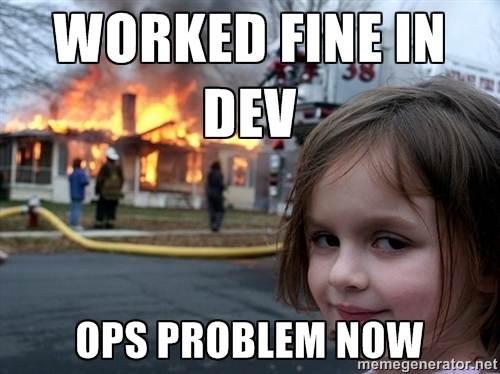
\includegraphics[width=0.8\textwidth]{images/devops.jpg}
\end{center}

\end{frame}



\begin{frame}
\frametitle{Start Me Up}

This is not the case at startup companies. 

There isn't the money to pay for separate developers and operations teams. 

And in the beginning there's probably not that many servers, just a few demo systems, test systems, etc... but it spirals out from there. 

You're not really going to ask the sales guys to manage these servers, are you? So, there's DevOps. 


\end{frame}



\begin{frame}
\frametitle{DevOps - Good Plan?}

Is DevOps a good idea? Like most ideas it can be used for both good and evil. 

There's a lot to be said for letting the developers be involved in all the parts of the software lifecycle.

Developers can learn a lot by having to do these kinds of things... 

And be motivated to make proper management and maintenance tools and procedures. 


\end{frame}



\begin{frame}
\frametitle{On the Other Hand...}

There's also something to be said for never letting the developers out of their cubes and keeping them far, far away from the customers. 

They will be scared. 

Both parties.


\end{frame}



\begin{frame}
\frametitle{Configuration as Code}

Systems have long come with complicated configuration options.


Sendmail is particularly notorious, but apache and nginx aren't super
easy to configure either.

The first principle is to treat \emph{configuration as code}.

\end{frame}



\begin{frame}
\frametitle{Configuration as Code}

\begin{itemize}
\item use version control on your configuration.
\item test your configurations.
\item aim for a suite of modular services that integrate together smoothly.
\item refactor configuration files.
\item use continuous builds (more on that later).
\end{itemize}

\end{frame}



\begin{frame}
\frametitle{Autoconfig}

Furthermore, it's an excellent idea to have tools for configuration. 

It's not enough to just have a wiki page or github document titled ``How to Install AwesomeApp'' (fill in name of program here). 

There are tons of great tools like the Red Hat Package Manager (RPM) which will allow you to make the installation and update process automatic and simple.

 Complicated means mistakes... people forget steps. They are human. 

\end{frame}



\begin{frame}
\frametitle{Servers as Cattle, not Pets}

By servers, I mean servers, or virtual machines, or containers.


At a certain scale (and it's smaller than you think), it's useful to
mass-produce tools for dealing with servers, rather than doing tasks
manually. 

At a minimum, you need to be able to set up these servers
without manual intervention. They should be able to be spun up 
programmatically.

\end{frame}



\begin{frame}
\frametitle{Common Infrastructure}

Use APIs to access your infrastructure. Some examples:

\begin{itemize}
\item storage: some sort of access layer to MongoDB or Amazon S3 or whatever;
\item naming and discovery infrastructure (more below);
\item monitoring infrastructure.
\end{itemize}

Try to avoid one-offs by using, for instance, open-source tools when applicable.
Be prepared to build your own tools if needed.


\end{frame}



\begin{frame}
\frametitle{Rule of Ten}

Consider eBay: in 1995, perl scripts; in 1997, C++/Windows; in 2002,
Java.  

Each of these architectures was appropriate at the time, but
not as the requirements change. 

The more sophisticated successor
architectures, however, would have been overkill at an earlier
time. 

And it's hard to predict what would be needed in the future.

\end{frame}



\begin{frame}
\frametitle{Perf}

\begin{quote}
``Perf is a feature''.\\
\hfill --- Jeff Atwood
\end{quote}
That is, you apply developer time to perf, and you make engineering tradeoffs
to get it. Some thoughts:
\begin{itemize}
\item design with the eventual replacement in mind;
\item don't abandon internal quality (e.g. modularity);
\item sacrifice individual modules at a time, not the whole system;
\item you can also implement new features with a rough draft and deploy to a test audience.
\end{itemize}



\end{frame}




\begin{frame}
\frametitle{Naming}

Naming is one of the hard problems in computing. 

There is a saying that there are only two hard things in computers: cache invalidation, naming things, and off by one errors. 

\end{frame}



\begin{frame}
\frametitle{Naming Suggestions}

\begin{itemize}
\item use canonical one-word names for servers;
\item but, use aliases to specify functions, e.g. 1) geography (nyc); 2) environment (dev/tst/stg/prod); 
3) purpose (app/sql/etc); and 4) serial number.
\end{itemize}


There's also the Java package approach of infinite dots: live.application.customer.webdomain.com or however you want to call it. 

Pick something and be consistent.

\end{frame}



\begin{frame}
\frametitle{Continuous Integration}

\begin{itemize}
\item pull code from version control;
\item build;
\item run tests;
\item report results.
\end{itemize}

What's also key is a social convention to not break the build. 

These things get done automatically on every commit and the results are sent to people by e-mail or instant messenger.

\end{frame}



\begin{frame}
\frametitle{Canarying}

\begin{center}
	
\includegraphics[width=0.9\textwidth]{images/blackcanary.jpg}
\end{center}

\end{frame}



\begin{frame}
\frametitle{Canarying}

Deploy new software incrementally alongside production software, also known as ``test in prod''. 


\begin{itemize}
\item stage for deployment;
\item remove canary servers from service;
\item upgrade canary servers;
\item run automatic tests on upgraded canaries;
\item reintroduce canary servers into service;
\item see how it goes!
\end{itemize}


Of course, you should implement your system so that rollback is possible.

\end{frame}



\begin{frame}
\frametitle{Monitoring}
Things to think about:

\begin{itemize}
	\item CPU Load
	\item Memory Utilization
	\item Disk Space
	\item Disk I/O
	\item Network Traffic
	\item Clock Skew
	\item Application Response Times
\end{itemize}


\end{frame}



\begin{frame}
\frametitle{Dashboard}

With multiple systems, you will want some sort of dashboard that gives an overview of all the multiple systems in a summary. 

The summary needs to be sufficiently detailed that you can detect if anything is wrong, but not an overwhelming wall of data. 

Then you do not necessarily want to pay someone to stare at the dashboard and press the  ``Red Alert!'' button if anything goes out of some preset range.

No, for that we need some automatic monitoring.


\end{frame}



\begin{frame}
\frametitle{Red Alert}

\begin{itemize}
\item {\bf Alerts}: a human must take action now;
\item {\bf Tickets}: a human must take action soon (hours or days);
\item {\bf Logging}: no need to look at this except for forensic/diagnostic purposes.
\end{itemize}


A common bad situation is logs-as-tickets.

\end{frame}



\begin{frame}
\frametitle{Action Stations! Set Condition One Throughout the Ship}

It is very important to be judicious about the use of alerts. 

If your alerts are too common, they get ignored. 

When you hear the fire alarm in a building, chances are your thought is not ``the building is on fire; I should leave it immediately in an orderly fashion.''.

It's a good heuristic; you'll be correct most of the time. 

But if there is an actual fire, you will not only be wrong, you might also be dead.

\end{frame}



\begin{frame}
\frametitle{Not the Kittens!!!}

Alerts and tickets are a great way to make user pain into developer pain.

Some SUPER CRITICAL ticket OMG KITTENS ARE ENDANGERED is an excellent way to learn the lesson... 

Devs will take steps that keep these things from happening in the future.

\end{frame}



\begin{frame}
\frametitle{Clusters vs Laptops}

The key idea: scaling to big data systems introduces substantial overhead. 

Let's just see how, say, a laptop compares, in absolute times, to 128-core big data systems.


\end{frame}



\begin{frame}
\frametitle{Clusters vs Laptops}

Big data systems haven't yet been shown to be obviously good; current evaluation is lacking.

The important metric is not just scalability; absolute
performance matters a lot. 

We don't want a situation where we are just scaling up to $n$ systems to deal with the complexity of scaling up to $n$ systems. 

Or, as Oscar Wilde put it: ``The bureaucracy is expanding to meet the needs of the expanding bureaucracy.''

\end{frame}



\begin{frame}
\frametitle{Methodology}

We'll compare a competent single-threaded implementation to top
big data systems. 

The domain: graph processing
algorithms, namely PageRank and graph connectivity (for which the bottleneck is label propagation). 

The subjects: graphs with billions of edges, amounting to a few
GB of data.


\end{frame}



\begin{frame}
\frametitle{Results}

\begin{center}
	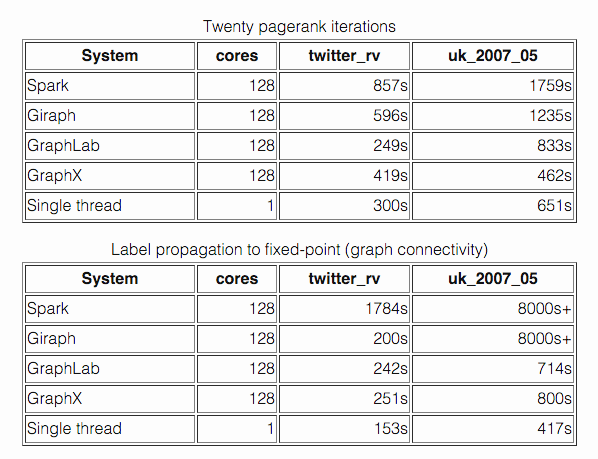
\includegraphics[width=0.80\textwidth]{images/pagerank.png}
\end{center}


\end{frame}



\begin{frame}
\frametitle{Takeaways}

\begin{itemize}
\item    ``If you are going to use a big data system for yourself, see if it is faster than your laptop.''
\item    ``If you are going to build a big data system for others, see that it is faster than my laptop.''
\end{itemize}


\end{frame}


\end{document}

